During the review of the summer results we decided to introduce an
additional selection requirement
$m_{T}^{\ell\ell\met}>80$~\GeV{}. This requirement was motivated by
lack of confidence in how well the low $m_{T}$ part is understood. In
particular this requirement makes the contribution of \dytt\
completely negligible and greatly reduce \wgamma\ contribution. Now we
have 3 times more data and as a cross-check it is useful to see how
well data and Monte Carlo agree in the low
$m_{T}$. Figures~\ref{fig:bdt_hww120}-\ref{fig:bdt_hww400} show BDT
MVA output for $m_{T}^{\ell\ell\met}<80$ events for a few key Higgs
mass hypotheses. In general we see a good agreement between data and
Monte Carlo. We may want to relax this requirement in the future
updates of the analysis.

\begin{figure}[!hbtp]
\centering
\subfigure[$e\mu$ 0-Jet]{
\centering
\label{subfig:bdt_hww120_0j_of}
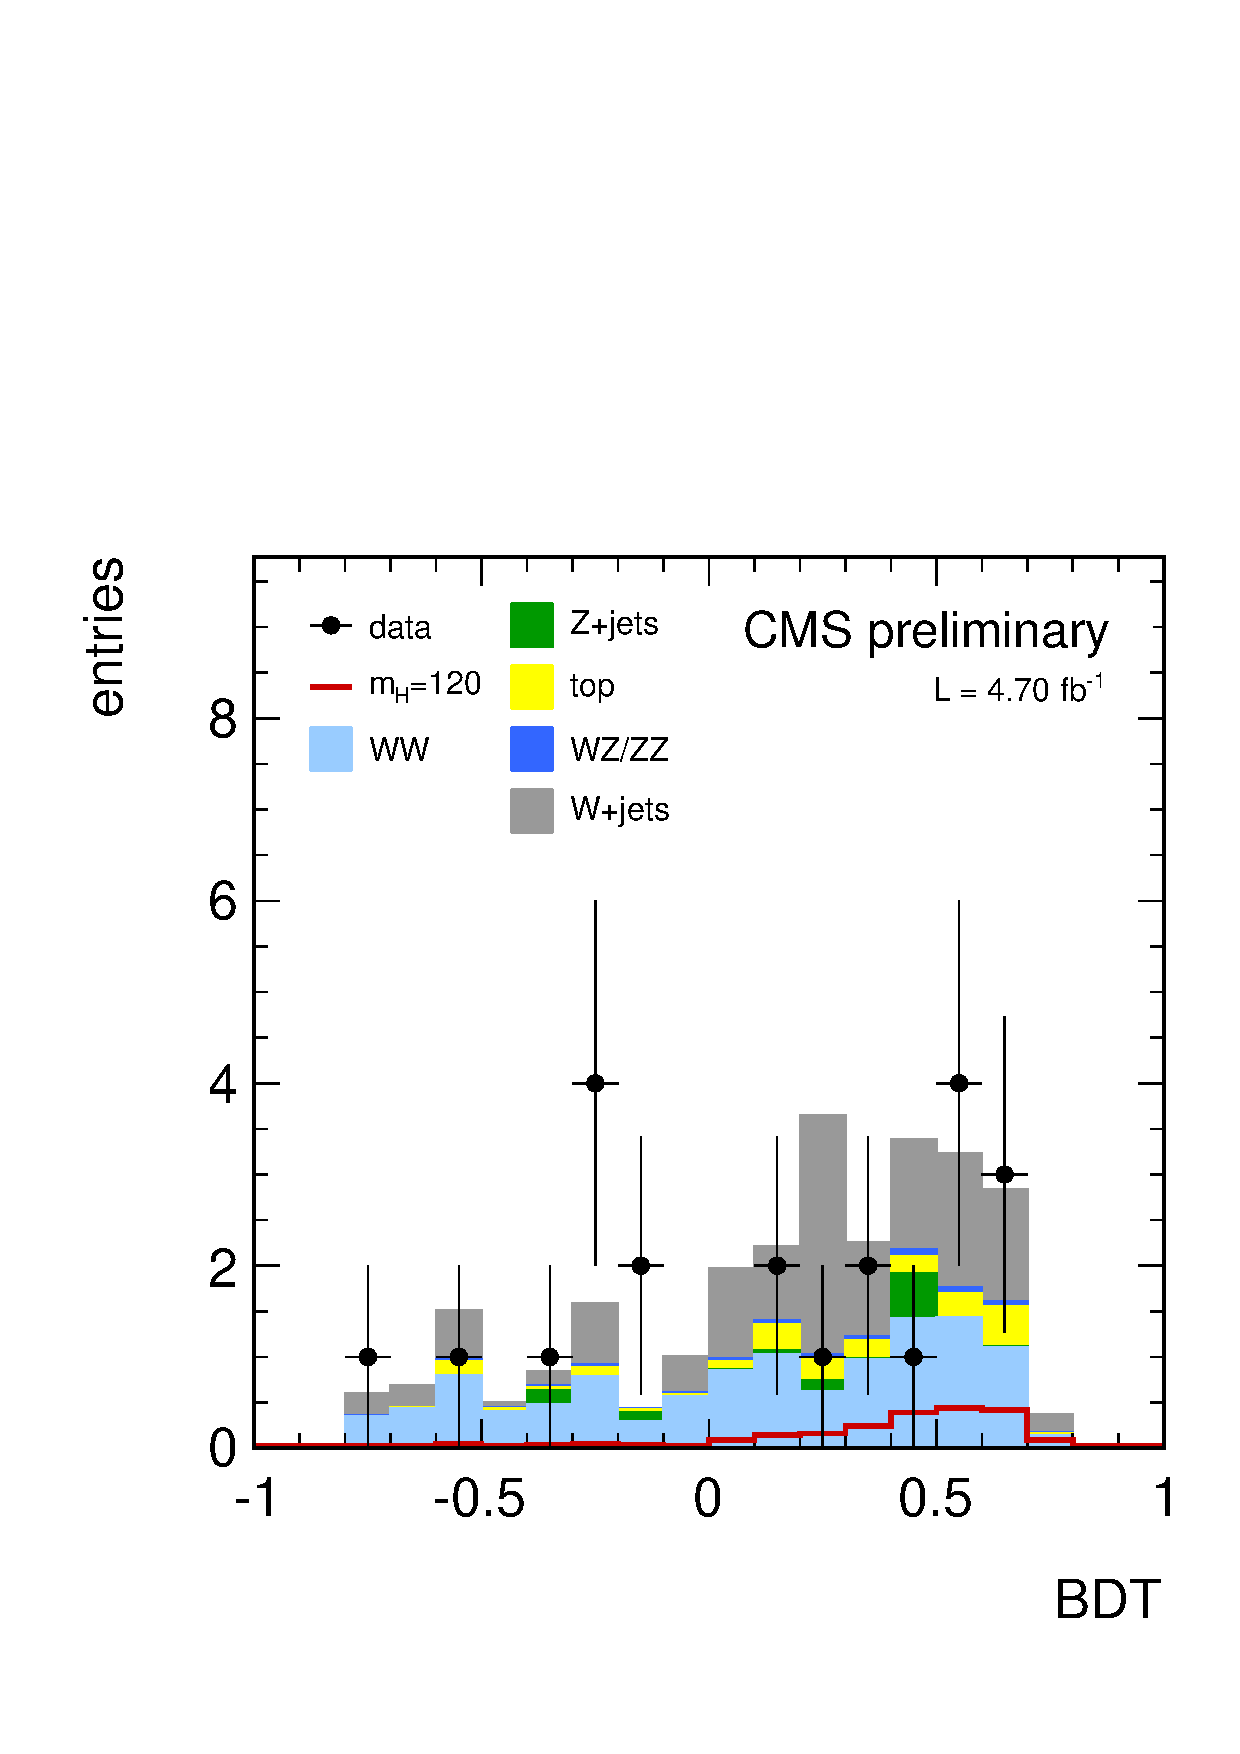
\includegraphics[width=.40\textwidth]{figures/bdt_hww120_0j_of.pdf}}
\subfigure[$ee$/$\mu\mu$ 0-Jet]{
\centering
\label{subfig:bdt_hww120_0j_sf}
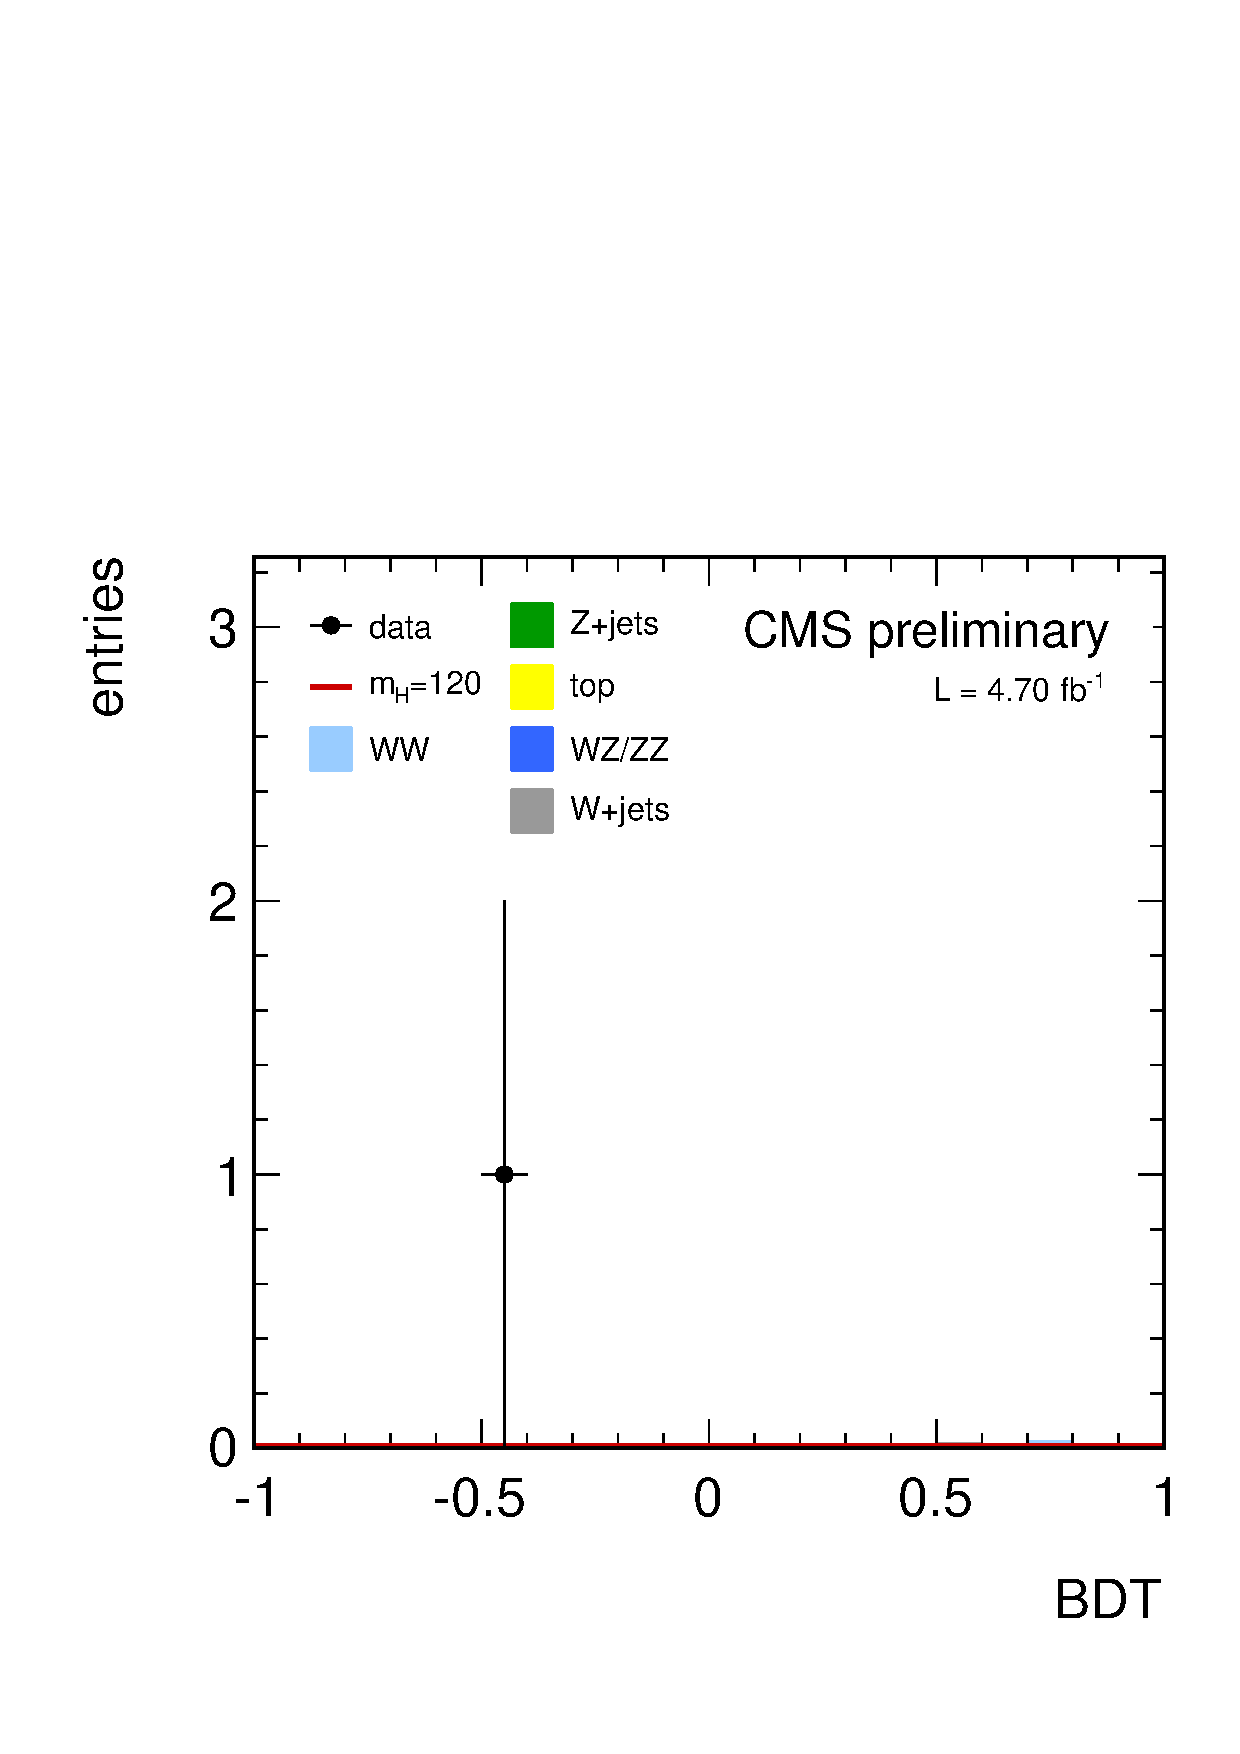
\includegraphics[width=.40\textwidth]{figures/bdt_hww120_0j_sf.pdf}}
\subfigure[$e\mu$ 1-Jet]{
\centering
\label{subfig:bdt_hww120_1j_of}
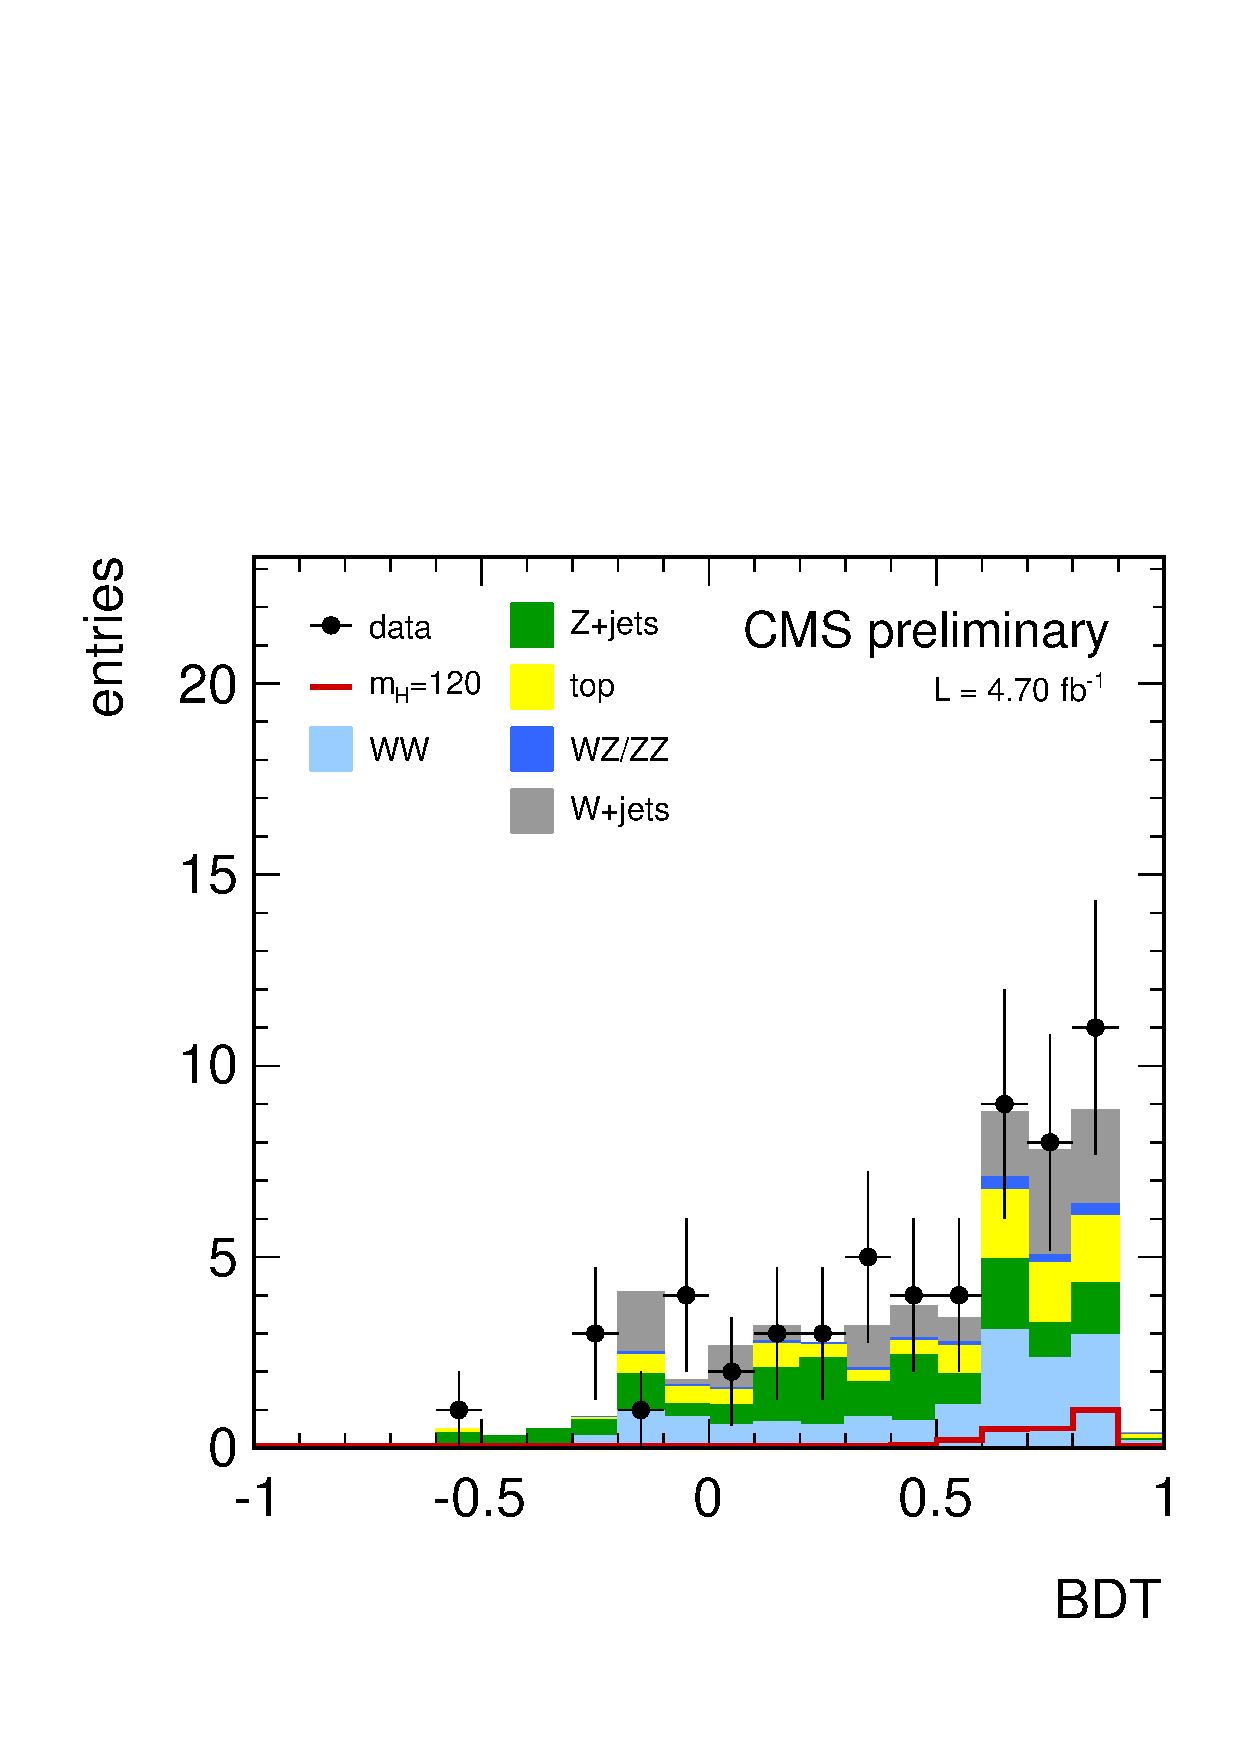
\includegraphics[width=.40\textwidth]{figures/bdt_hww120_1j_of.pdf}}
\subfigure[$ee$/$\mu\mu$ 1-Jet]{
\centering
\label{subfig:bdt_hww120_1j_sf}
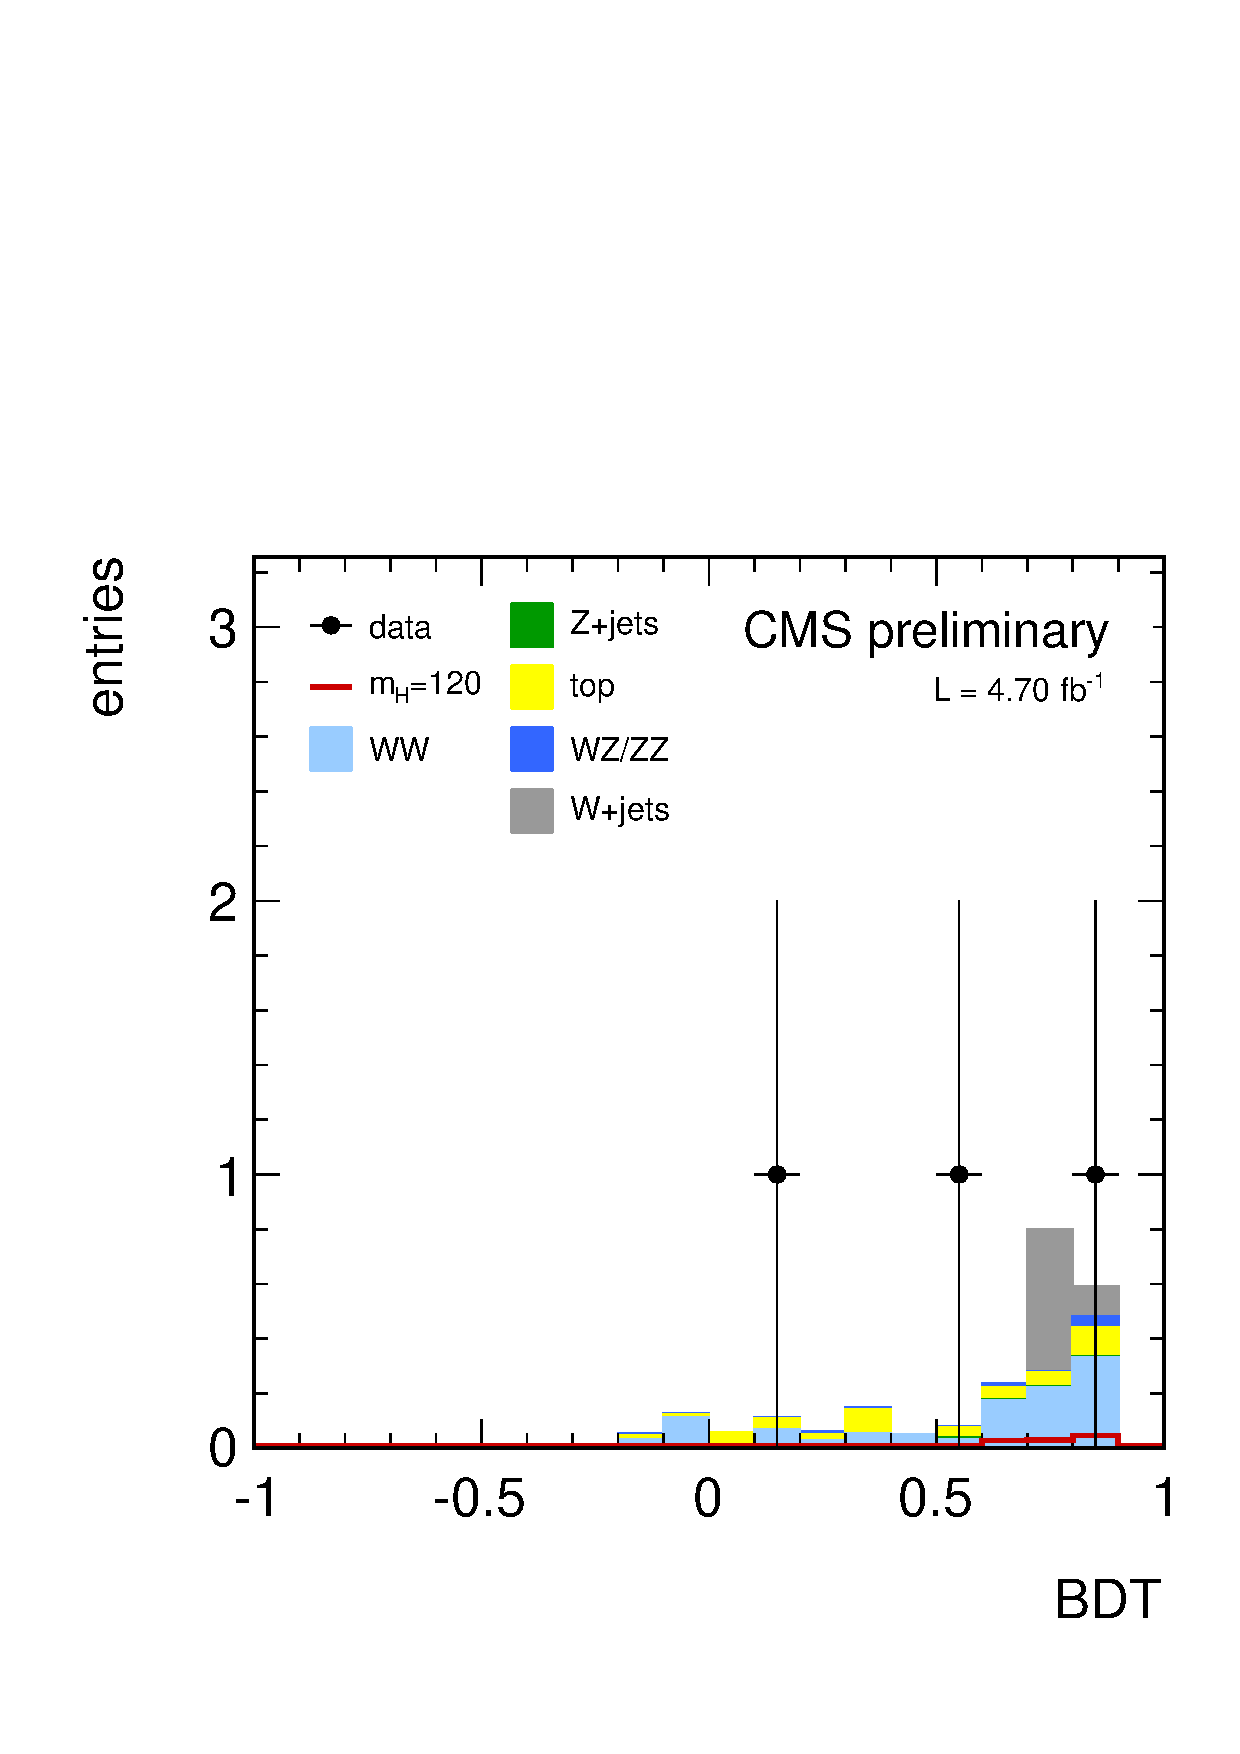
\includegraphics[width=.40\textwidth]{figures/bdt_hww120_1j_sf.pdf}}
\caption{
BDT MVA output optimized for {\bf 120~\GeV\ Higgs mass} point for events
with $m_{T}^{\ell\ell\met}<80$ corresponding to \intlumi{}.  }
\label{fig:bdt_hww120}
\end{figure}

\begin{figure}[!hbtp]
\centering
\subfigure[$e\mu$ 0-Jet]{
\centering
\label{subfig:bdt_hww130_0j_of}
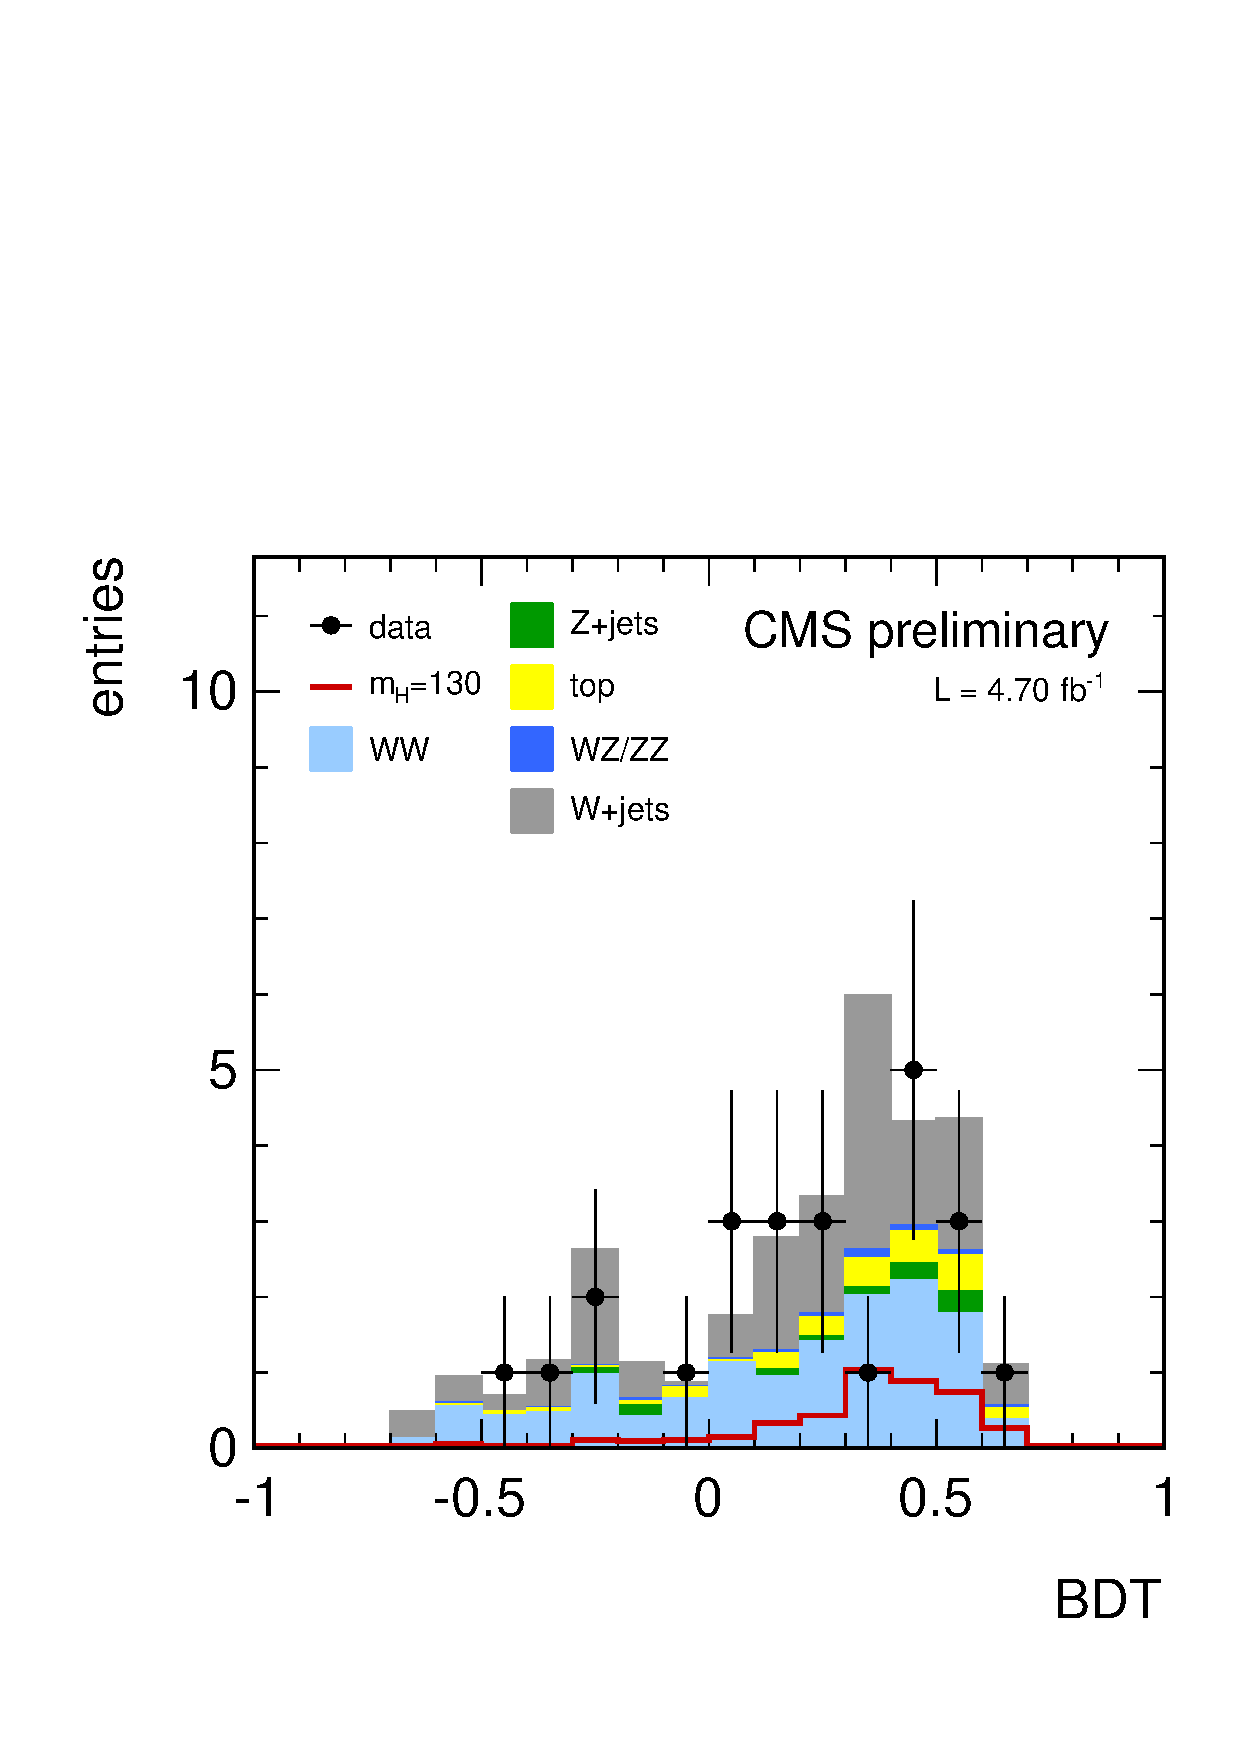
\includegraphics[width=.40\textwidth]{figures/bdt_hww130_0j_of.pdf}}
\subfigure[$ee$/$\mu\mu$ 0-Jet]{
\centering
\label{subfig:bdt_hww130_0j_sf}
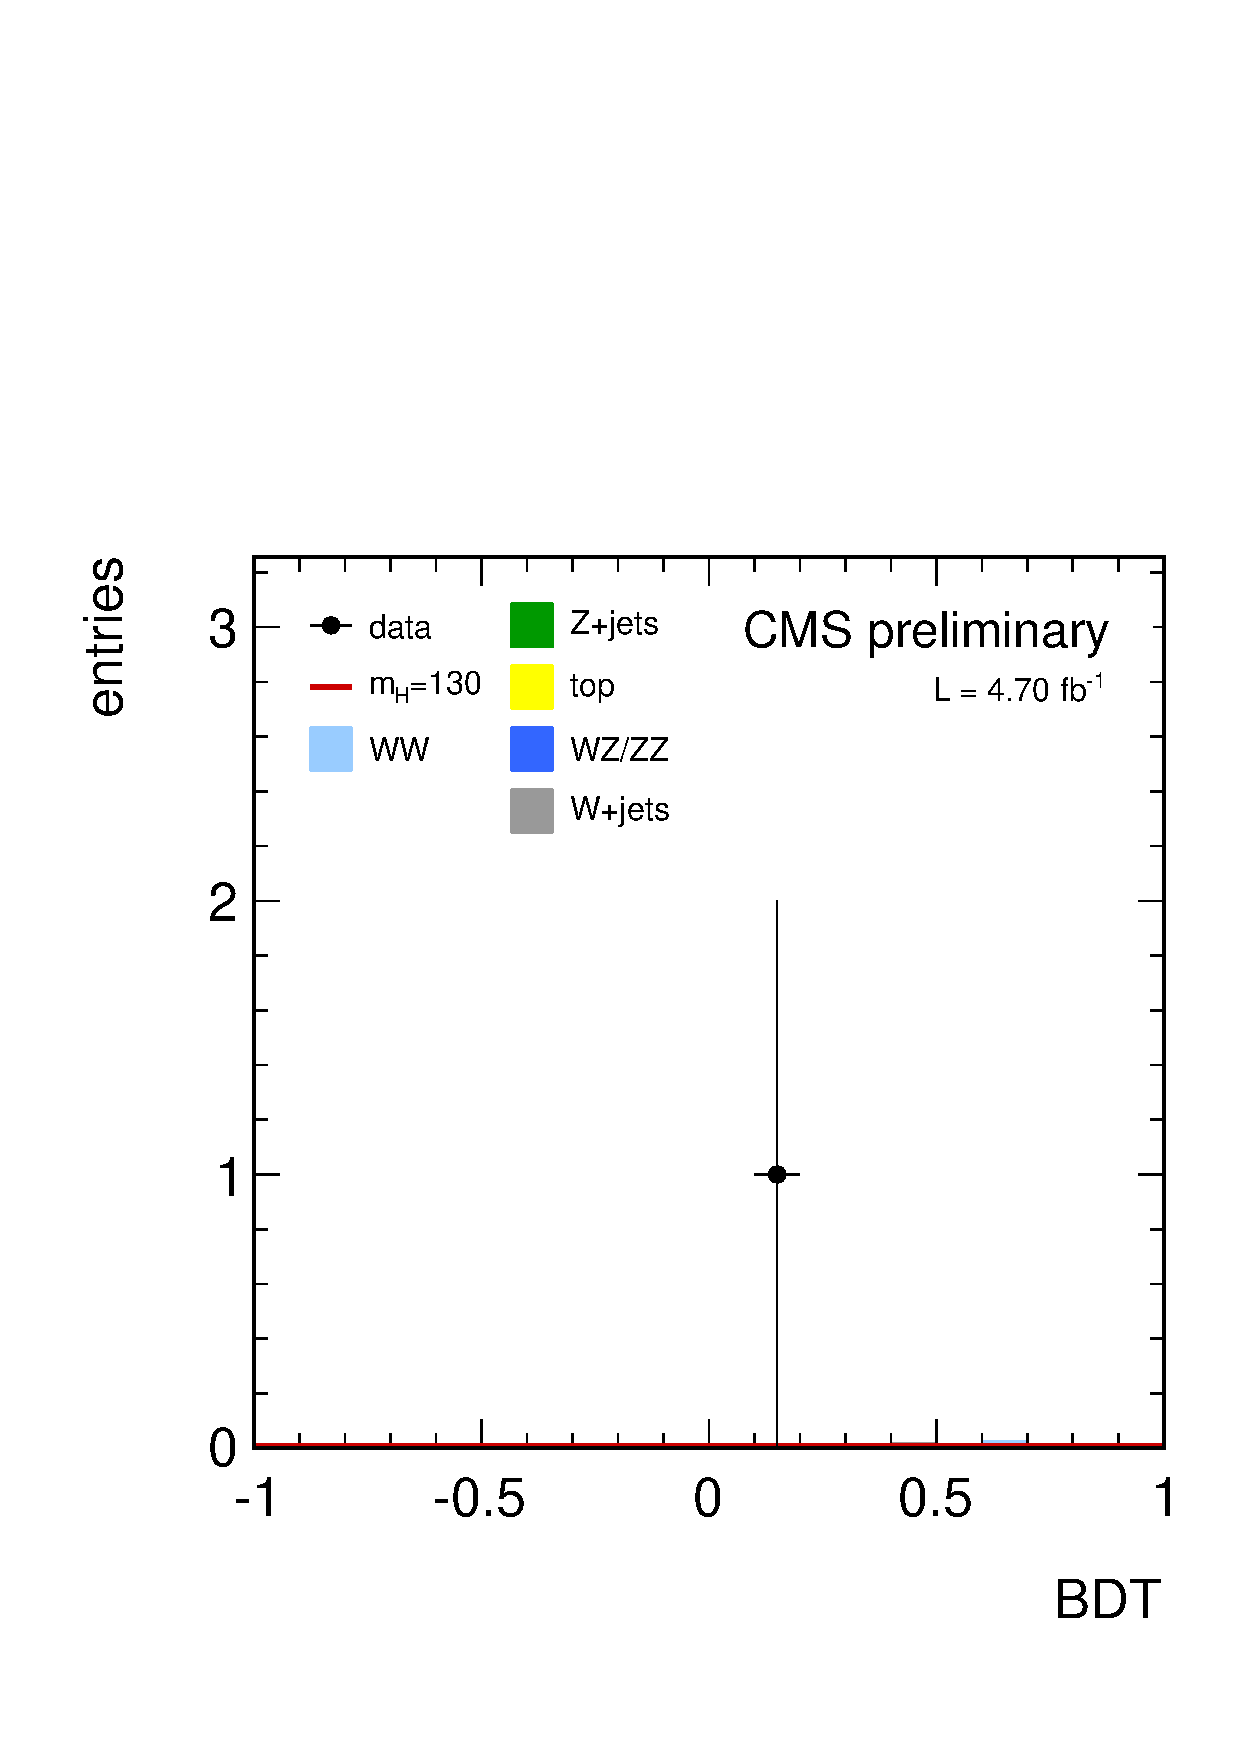
\includegraphics[width=.40\textwidth]{figures/bdt_hww130_0j_sf.pdf}}
\subfigure[$e\mu$ 1-Jet]{
\centering
\label{subfig:bdt_hww130_1j_of}
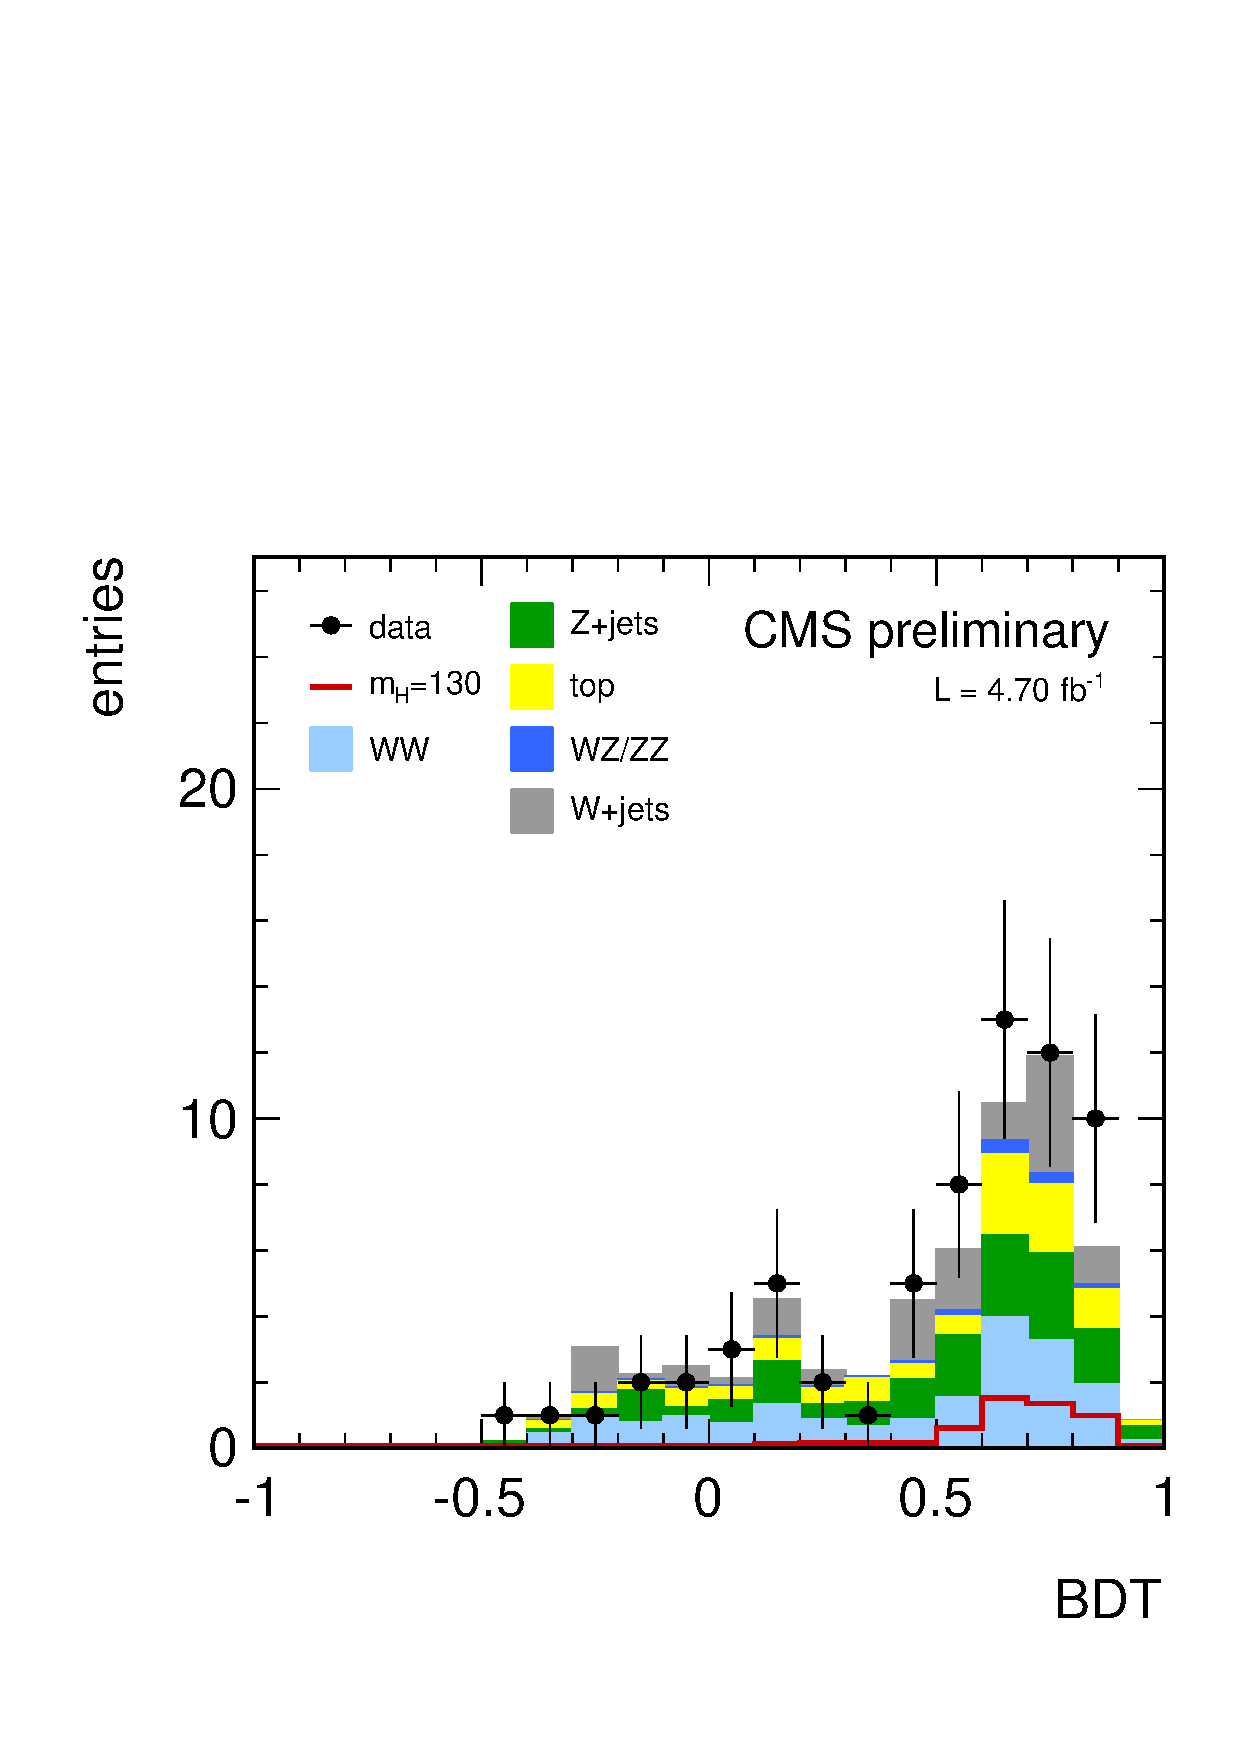
\includegraphics[width=.40\textwidth]{figures/bdt_hww130_1j_of.pdf}}
\subfigure[$ee$/$\mu\mu$ 1-Jet]{
\centering
\label{subfig:bdt_hww130_1j_sf}
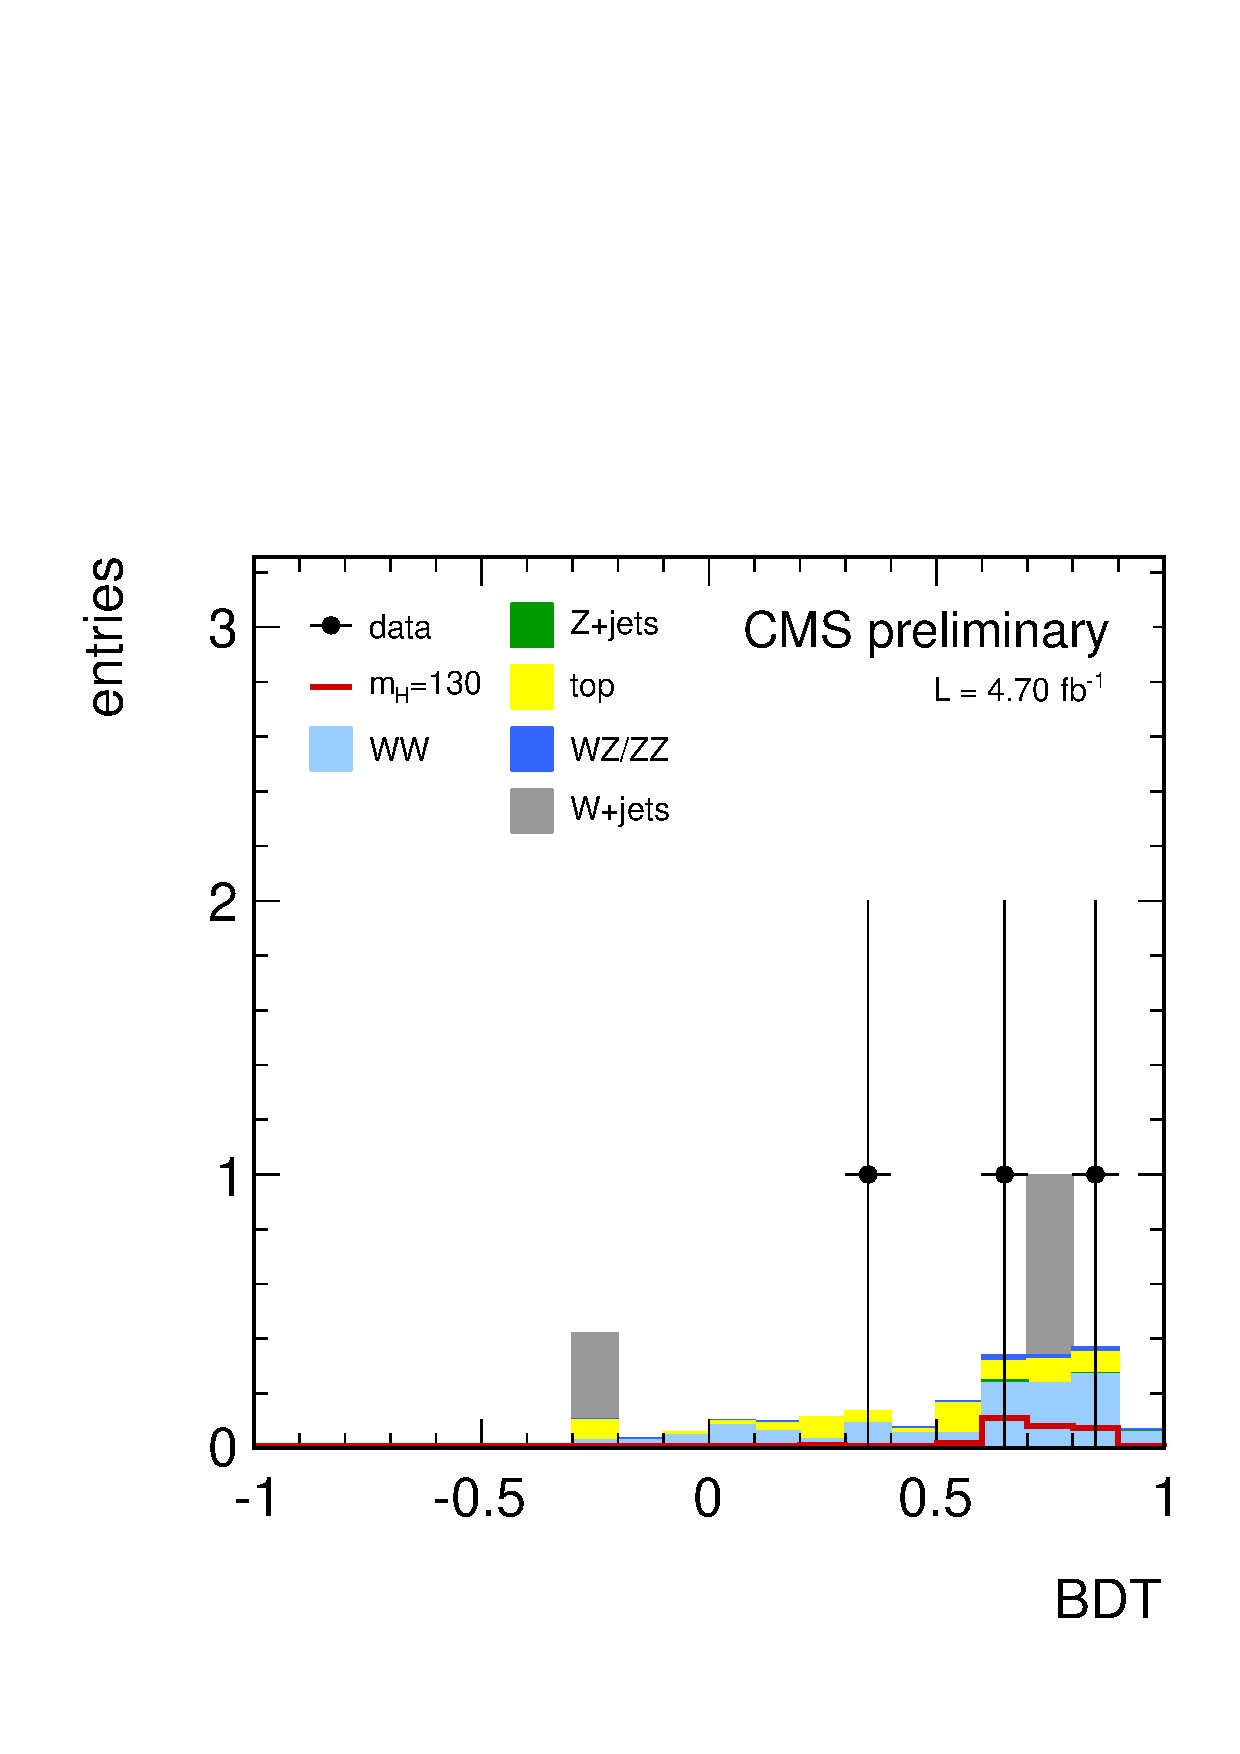
\includegraphics[width=.40\textwidth]{figures/bdt_hww130_1j_sf.pdf}}
\caption{
BDT MVA output optimized for {\bf 130~\GeV\ Higgs mass} point for events
with $m_{T}^{\ell\ell\met}<80$ corresponding to \intlumi{}.  }
\label{fig:bdt_hww130}
\end{figure}

\begin{figure}[!hbtp]
\centering
\subfigure[$e\mu$ 0-Jet]{
\centering
\label{subfig:bdt_hww400_0j_of}
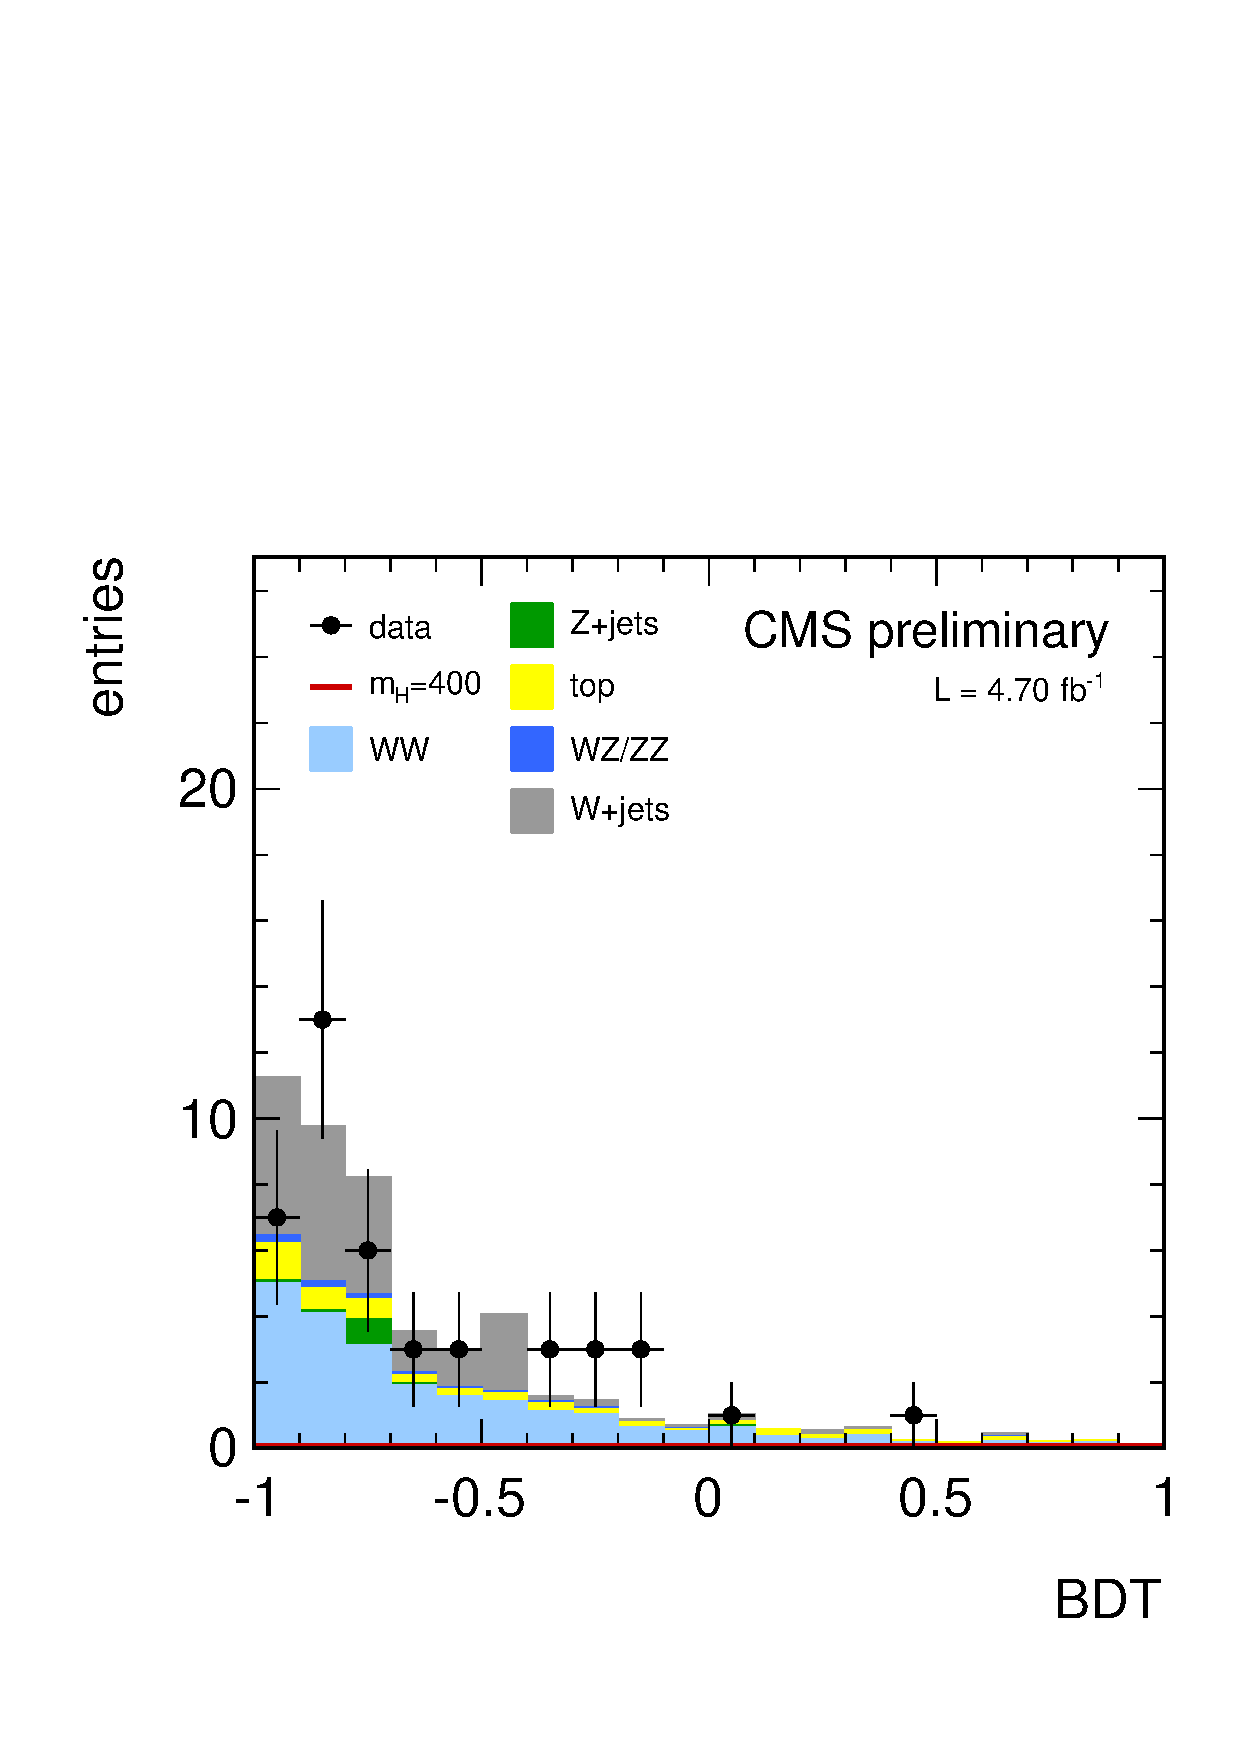
\includegraphics[width=.40\textwidth]{figures/bdt_hww400_0j_of.pdf}}
\subfigure[$ee$/$\mu\mu$ 0-Jet]{
\centering
\label{subfig:bdt_hww400_0j_sf}
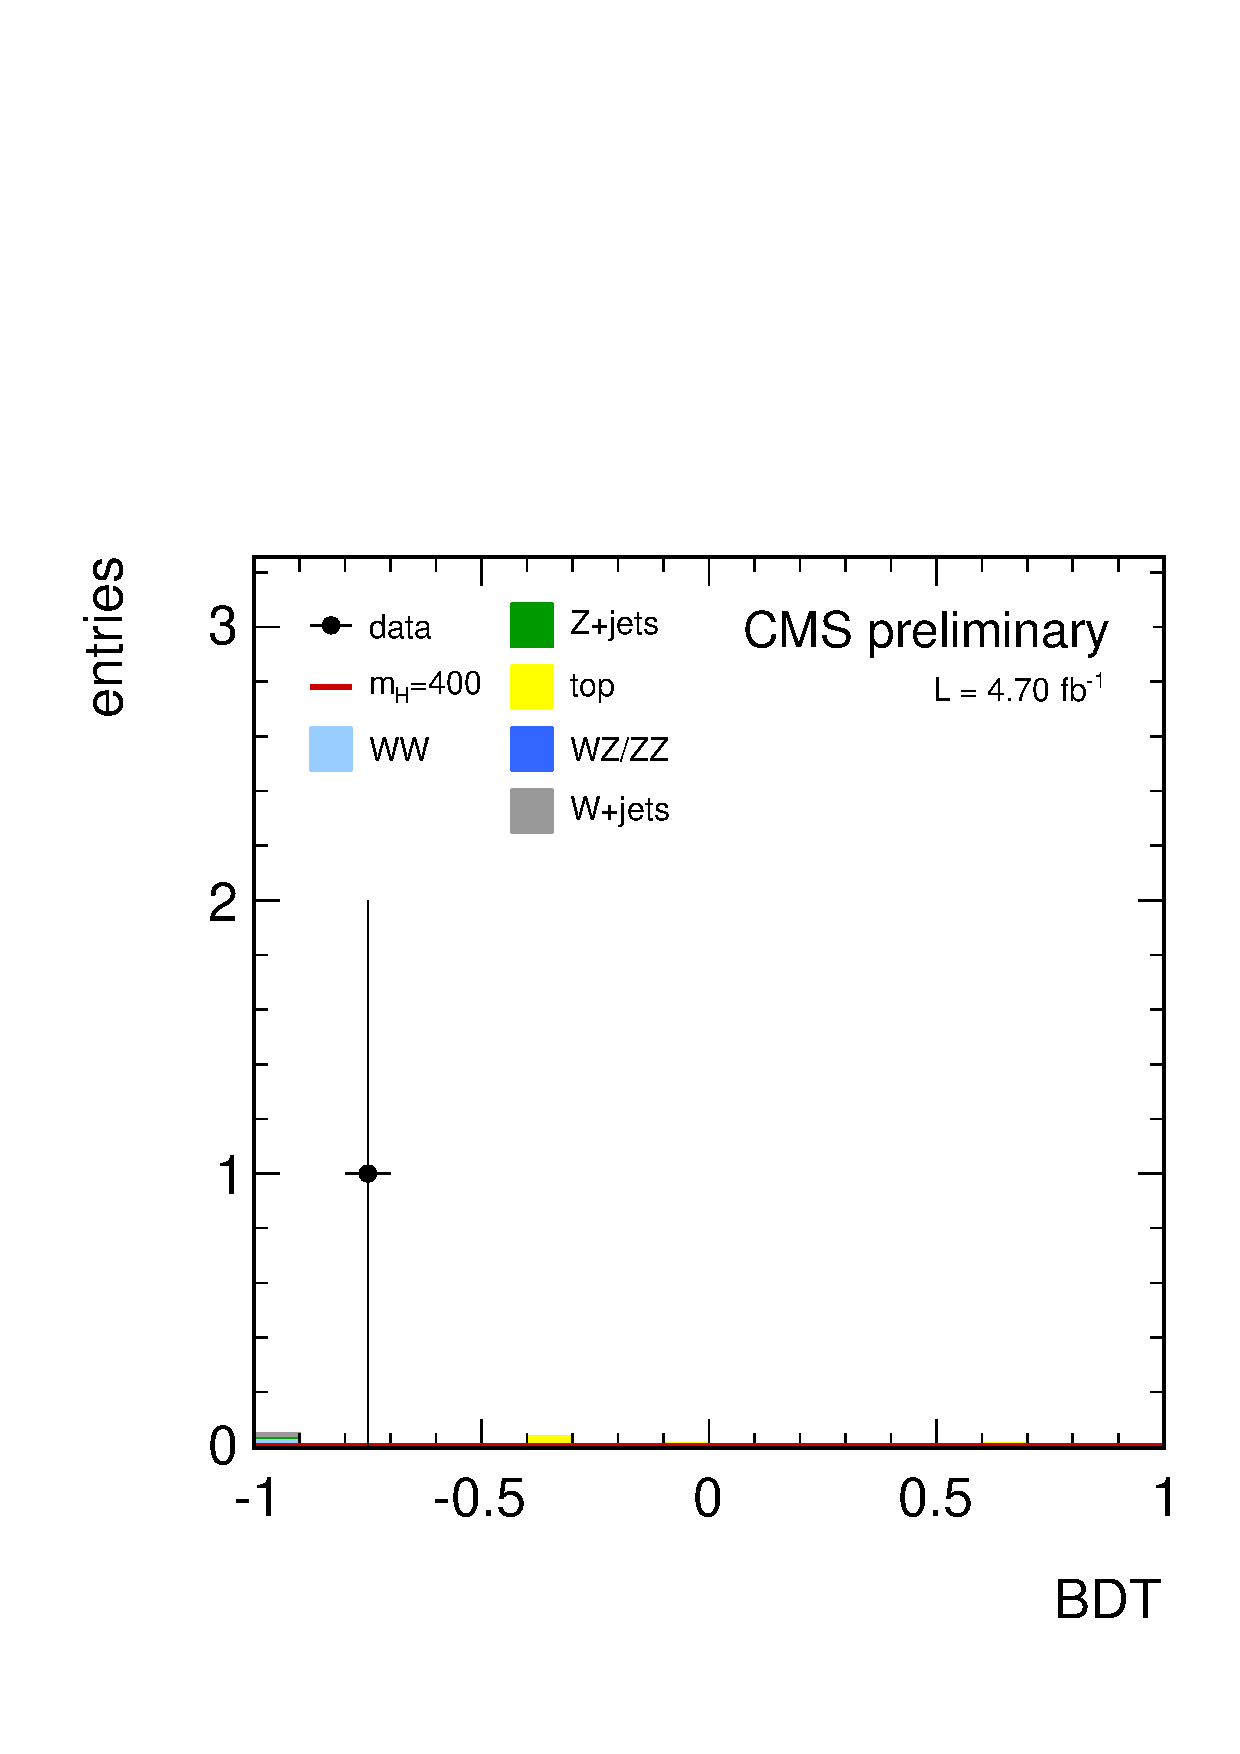
\includegraphics[width=.40\textwidth]{figures/bdt_hww400_0j_sf.pdf}}
\subfigure[$e\mu$ 1-Jet]{
\centering
\label{subfig:bdt_hww400_1j_of}
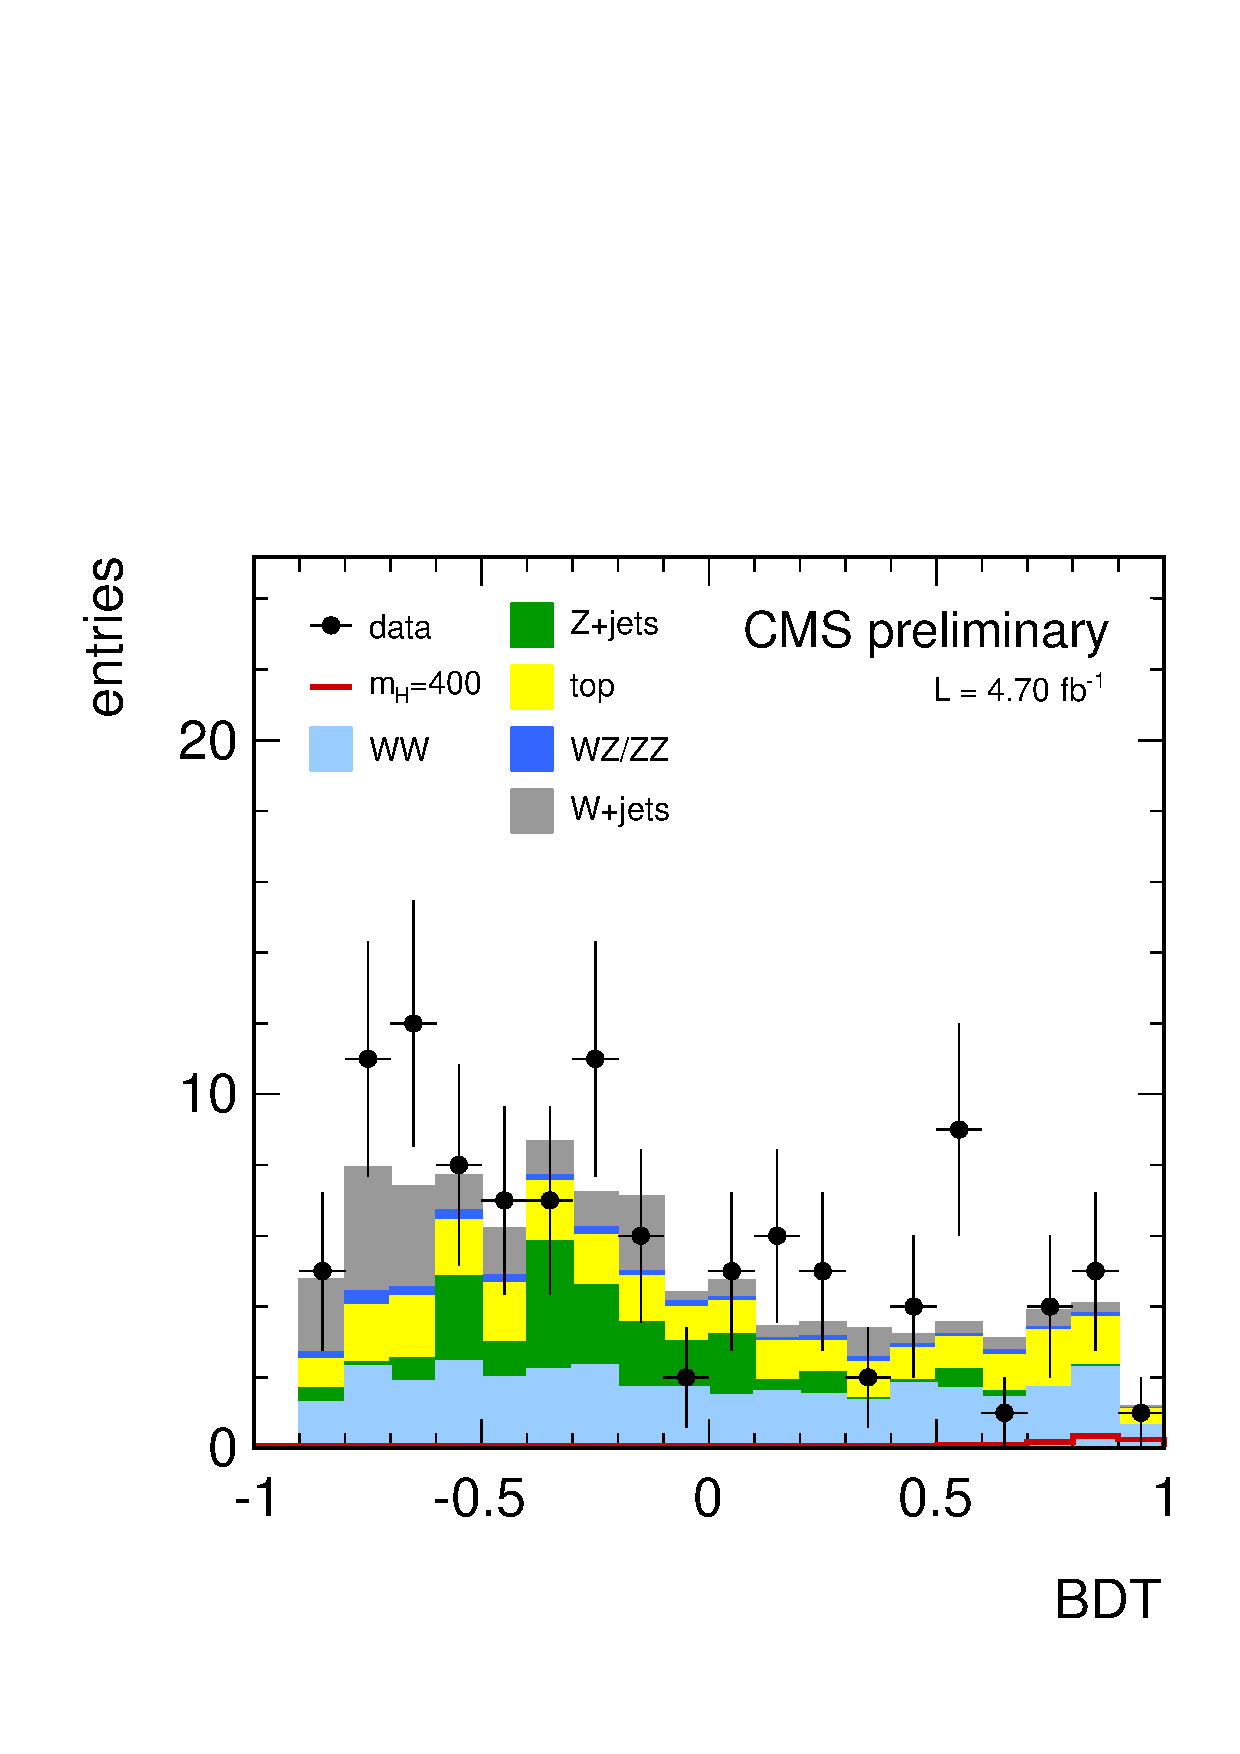
\includegraphics[width=.40\textwidth]{figures/bdt_hww400_1j_of.pdf}}
\subfigure[$ee$/$\mu\mu$ 1-Jet]{
\centering
\label{subfig:bdt_hww400_1j_sf}
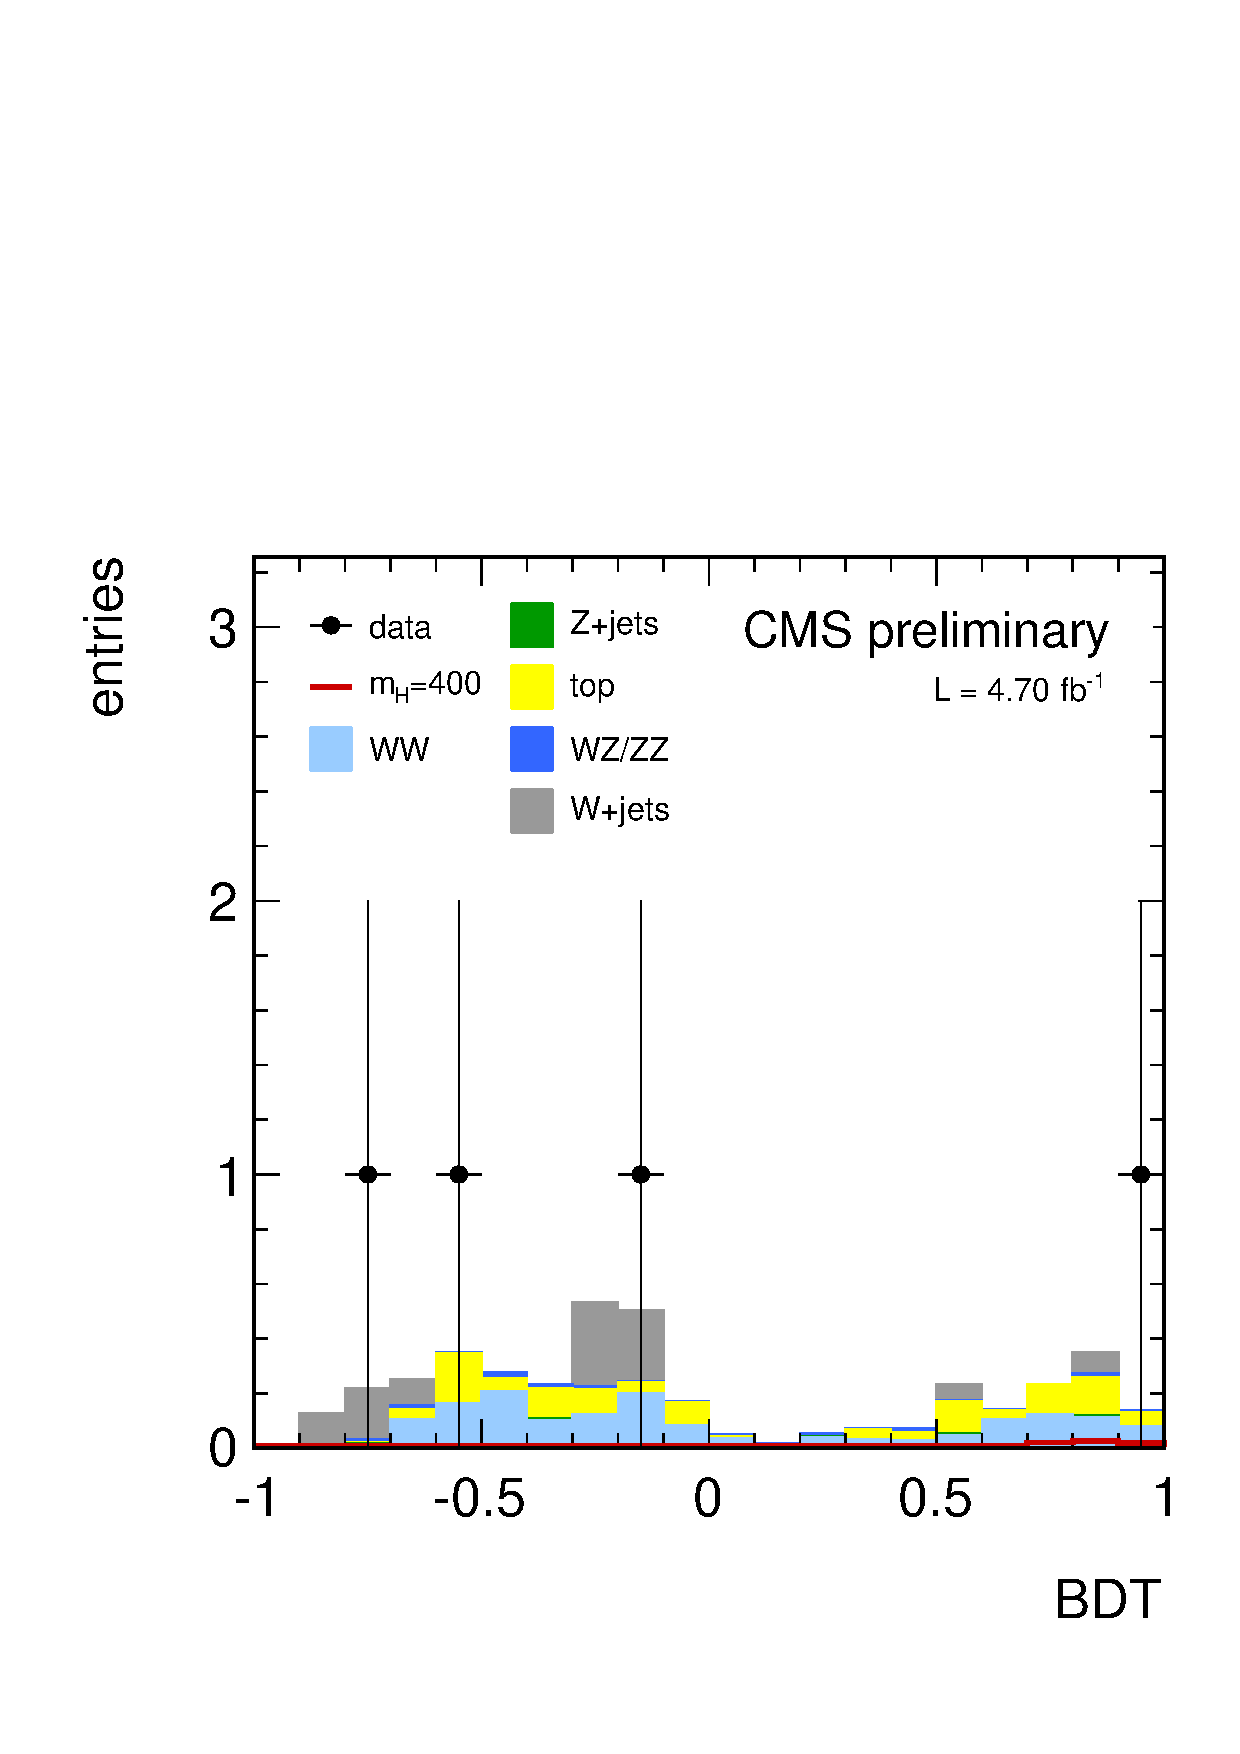
\includegraphics[width=.40\textwidth]{figures/bdt_hww400_1j_sf.pdf}}
\caption{
BDT MVA output optimized for {\bf 400~\GeV\ Higgs mass} point for events
with $m_{T}^{\ell\ell\met}<80$ corresponding to \intlumi{}.  }
\label{fig:bdt_hww400}
\end{figure}
